\documentclass[12pt]{article}
\usepackage{amsmath}
\usepackage{amsfonts}
\usepackage{amssymb}
\usepackage{amsthm}
\usepackage{amsmath}
\usepackage{verbatim}
\usepackage{bbm}
\usepackage{bm}
\usepackage{braket}
\usepackage{graphicx}
\usepackage{subfig}

\usepackage[shortlabels]{enumitem}
\usepackage[margin=1in]{geometry}
%\setlength{\parindent}{0cm}

\newcommand{\varep}{\varepsilon}
\newcommand{\N}{\mathbb{N}}
\newcommand{\Z}{\mathbb{Z}}
\newcommand{\Q}{\mathbb{Q}}
\newcommand{\R}{\mathbb{R}}
\newcommand{\C}{\mathbb{C}}
\newcommand{\Id}{\mathbbm{1}}
\newcommand{\lnskip}{\vspace{\baselineskip}}
\newcommand{\oln}{\overline}
\renewcommand{\Re}{\mathrm{Re}}
\renewcommand{\Im}{\mathrm{Im}}
\newcommand{\Int}{\mathrm{Int}}
\newcommand{\Arg}{\mathrm{Arg}}

\title{Plane-waves at the interface between two-dimensional cyclic Lotka-Volterra and May-Leonard systems}
\author{M. Lazarus Arnau\\ PHYS 4316 Modern Experimental Physics}

\hfuzz=6.8pt
\begin{document}

\maketitle

\begin{abstract}
    The spatially extended May-Leonard model for cyclic competition is known 
    to demonstrate (quasi-)stable spatio-temporal patterns in the form of
    spiral-waves. We investigate how competition between the May-Leonard model 
    and cyclic Lotka-Volterra models governing different spatial regions of a 
    two-dimensional system influences the formation of spiral-waves. To this end
    we employ a lattice-based Monte-Carlo simulation. We report disruption of the
    spiral-waves near the interface for certain mobility rates in the cyclic Lotka-Volterra
    region. We quantify the behavior of these plane-waves by computing the vertical
    auto-correlation functions. We also report a significant decrease in local
    population density near the interface.
\end{abstract}
\section{Introduction}%
\label{sec:introduction}

Many systems across nature follow a cyclic, or Rock-Paper-Scissors (RPS) like, 
paradigm of competition. As such, cyclic competition models have been used to 
describe the evolutionary dynamics and noise-induced pattern formation in such systems 
(e.g. certain species of side-blotched lizards\cite{lizards}, in-vitro experiments performed on colonies of \textit{E. coli}
bacteria \cite{ecoli}, and the Belousov-Zhobatinsky reaction \cite{bz}). Two variations
of three-species competition models that have been extensively studied are the 
May-Leonard model and cyclic Lotka-Volterra model \cite{dobromasyletal}. 
Of note is that in its spacially extended variant the May-Leonard model has 
been shown to demonstrate noise-induced spatio-temporal pattern formation whereas
the cyclic Lotka-Volterra model does not \cite{dobromasyletal}.

Our goal in this paper is to investigate how competition between the cyclic Lotka-Volterra 
and May-Leonard models impacts the spatio-temporal dynamics demonstrated by the 
May-Leonard model. To that end, we describe a stochastic spatially-extended 
lattice based system which is governed by the two models on different spatial regions
of the lattice. We implement a Monte-Carlo simulation of this system and report 
the results of the simulations. We describe the formation of plane-waves at the
interface between the two models and quantify their formation by coputing the 
vertical auto-correlation function. We also report a drop in local population 
density near the interface.





\section{Our system}%
\label{sec:our_system}


\subsection{The May-Leonard and Cyclic Lotka-Volterra models}%
\label{sub:models}

The May-Leonard model (MLM) and cyclic Lotka-Volterra models both describe systems 
in which the population obeys a cyclic (or Rock-Paper-Scissors) competition scheme. 
Individuals are thus modeled as particles which can be one of three species, 
$ S \in \set{S_1, S_2, S_3} $ with the cyclic symmetry $ S_4 = S_1 $. These particles
are equipped with different reactions.
The original May-Leonard (MLM) model defines two reactions, predation and reproduction:
\begin{align}
    \label{eq:mlpred} S_n + S_{n+1} \to S_n + \emptyset \qquad &\text{with rate } \sigma\\
    \label{eq:mlrep} S_n + \emptyset \to S_n + S_n \qquad &\text{with rate } \beta
\end{align}
The cyclic Lotka-Volterra model (CLVM) defines a single predation and reproduction reaction:
\begin{equation}
    \label{eq:rpspred} S_n + S_{n+1} \to S_n + S_n \qquad \text{with rate } \zeta
\end{equation}
A particle can move from its current node $ \bm{x} $ to one of its nearest neighbors
$ \bm{x}'$ via a mobility process
\begin{equation}
    \label{eq:mob} X_{\bm{x}} + Y_{\bm{x}'} \to Y_{\bm{x}} + X_{\bm{x}'} \qquad \text{with rates } \delta_{\mathrm{CLV}} \text{ and } \delta_{\mathrm{ML}}
\end{equation}
Where $ X \in \set{S_1. S_2, S_3} $ and $ Y \in \set{\emptyset, S_1. S_2, S_3} $. It is common to have two different reactions
for pair-exchanges (between active nodes) and diffusion (in to empty nodes) \cite{dobromasyletal}. By combining the two processes 
we are merely simplifying to the case in which the pair-exchange rate is equal to the diffusion rate.

Mean field analysis of a pure CLVM system reveals a marginally stable reactive fixed point of 
$ \bm{\rho}_{\mathrm{CLV}}^* = (\rho/3, \rho/3, \rho/3) $ where 
$ \rho = \rho_1(t) + \rho_2(t) + \rho_3(t) $ is a conserved quantity\cite{HeTauberZia}.
The CLVM also admits three unstable two-species extinction absorbing states \cite{HeTauberZia}.
Similar analysis of the MLM reveals a reactive fixed point $ \bm{\rho}_{\mathrm{ML}}^* = \frac{\beta}{3\beta + \sigma}(1,1,1) $ 
as well as four unstable absoring states $ \bm{\rho} = (1,0,0) $, $ (0,1,0) $, $ (0,0,1) $, and
$ (0,0,0) $ \cite{HeMobiliaTauber}. 

\begin{figure}[h]
    \begin{center}
    \subfloat[]
    {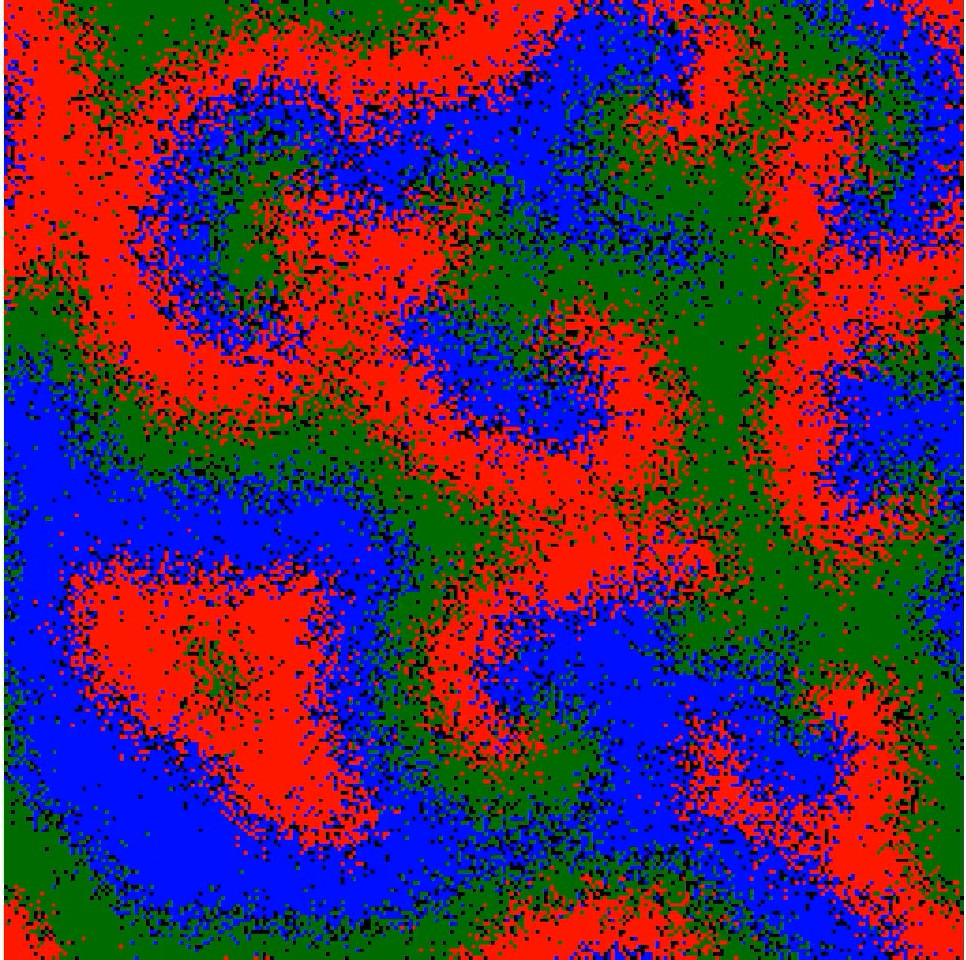
\includegraphics[width=0.45\linewidth]{images/ml_5_0.jpg}}
    \subfloat[]
    {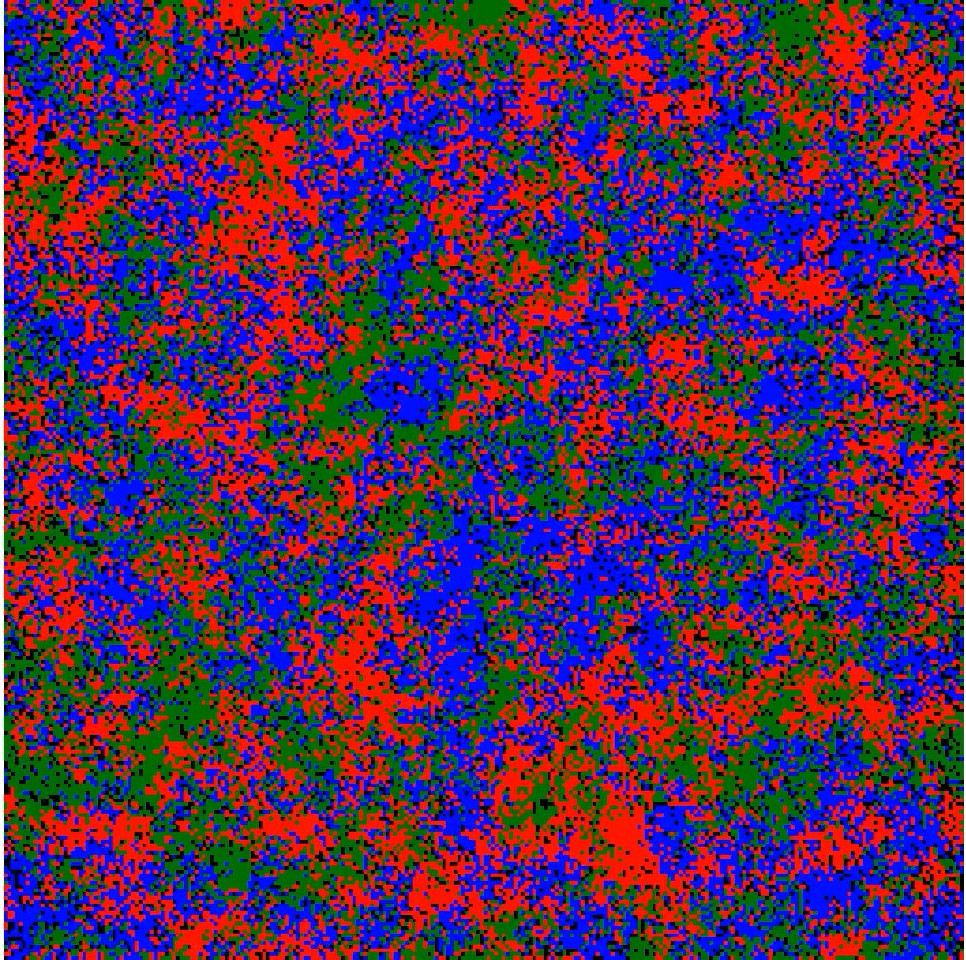
\includegraphics[width=0.45\linewidth]{images/rps_1_25.jpg}}\\
    \caption{Snapshots of typical behavior of the spatially extended May-Leonard (a) and cyclic Lotka-Volterra (b) models on
        a simulation of a $ 256\times 256 $ lattice. The rates used in the simulations for these images are $ \sigma = \beta = \zeta =1.0 $, $ \delta_{\mathrm{ML}} = 5.0$, and $ \delta_{\mathrm{CLV}} = 1.25 $    }
\label{fig:stab}
    \end{center} 
\end{figure}

The spatially extended versions of these two models exhibit drastically different behaviors. The MLM will produce distinctive spiral
waves whose size $ \ell $  is determined by $ \delta_{\mathrm{ML}} $ \cite{HeMobiliaTauber}. These waves are quasi-stable, remaining
present for very long time scales as long as the diffusivity of the system $ D = \delta_{\mathrm{ML}}/M^2 $ (where $ M $ is the
side length of the lattice) stays under a critical threshold $ D_c $ at which point the probability with which the system reaches 
one of the two-species extinction absorbing states rapidly approaches 1. The CLVM, while it will also maintain a quasi-stable stationary state around the coexistence 
fixed point it does not show any form of spatial pattern formation\cite{dobromasyletal}.

\subsection{Monte-Carlo simulation}%
\label{sub:monte_carlo_simulation}

\begin{figure}[h]
    \centering
    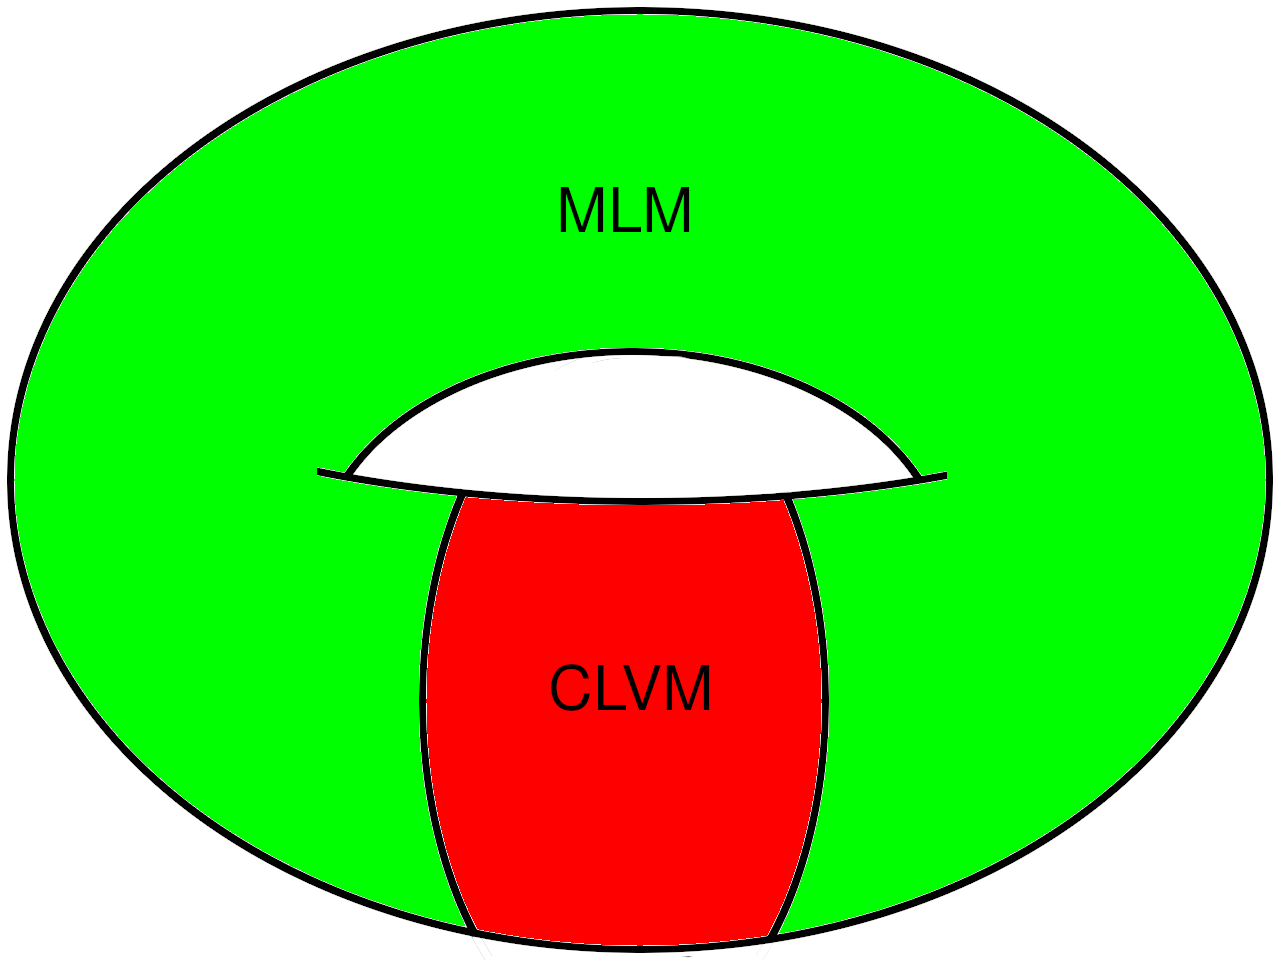
\includegraphics[width=0.5\linewidth]{images/Model_Illustration.png} 
    \caption{A schematic diagram illustrating the topology of the lattice and the ring shaped CLVM patch} \label{fig:schematic}
\end{figure}

We simulate our system on a lattice of size $ N = M \times M $  with periodic boundary conditions. 
In mixed model simulations, the lattice is governed primarily by the ML model reactions (\ref{eq:mlpred}, \ref{eq:mlrep}, \ref{eq:mob}) 
with the CLV model reactions (\ref{eq:rpspred}) and (\ref{eq:mob})  being imposed on the region 
$ \set{(x,y): 0\leq x\leq W} $ where a width of $ W = 64$ lattice nodes is normally used.
This makes those interface between the CLVM region and the ML region a continuous vertical line that wraps around the 
toroidal lattice like a ring. This allows us to calculate quantities averaged over columns parallel to the interface, 
the benefit of which will be apparent. 

The lattice is initialized to random, homogeneous initial conditions with $ \bm{\rho} = (0.3,0.3,0.3) $. At each simulation step
an active particle is selected by drawing random lattice nodes $ \bm{x} $ until a nonempty node is selected. Then one of the
four nearest neighbors $ \bm{x}' $ is selected at random. A reaction is then chosen at random from the model governing $ \bm{x} $. 
The probability with which a reaction is chosen is given by its rate divided by the sum of all rates defined by the given model.
So for instance, the probability that predation is chosen if $ \bm{x} $ is in the ML region of the lattice is 
$ \frac{\sigma}{\sigma + \beta + \delta_{\mathrm{ML}}}  $. 
%$ \sigma' = \sigma/\tau_{\mathrm{ML}} $, $ \beta' = \beta/\tau_{\mathrm{ML}} $, $ \delta_{\mathrm{ML}}' = \delta_{\mathrm{ML}}/\tau_{\mathrm{ML}} $,
%$ \zeta' = \zeta/\tau_{\mathrm{CVL}} $, and $ \delta_{\mathrm{CLV}}/\tau_{\mathrm{CLV}} $ where $ \tau_{\mathrm{ML}} = 
%\sigma + \beta + \delta_{\mathrm{ML}}$ and $ \tau_{\mathrm{CLV}} = \zeta + \delta_{\mathrm{CLV}} $ are normalization 
%factors. 
If the reaction chosen isn't possible with the chosen nearest neighbor the time step is still counted and a new 
$ \bm{x} $ and $ \bm{x}' $ are chosen. We define one Monte-Carlo step (MCS) to be the amount of time it takes on average for 
every particle to have an opportunity to react or migrate. Each MCS is thus composed of $ N $ infinitesimal simulation steps.

Unless noted otherwise the simulations are performed on a $ 512 \times 512 $ lattice with rates $ \sigma = \beta = \zeta =1.0 $, $ \delta_{\mathrm{ML}} = 5.0$, and $ \delta_{\mathrm{CLV}} = 1.25 $.


\section{Monte Carlo simulation results}%
\label{sec:monte_carlo_simulation_results}

\begin{figure}[!htb]
    \begin{center}
    \subfloat[ $ \delta_{\mathrm{CLV}} = 2.5 $ ]
    {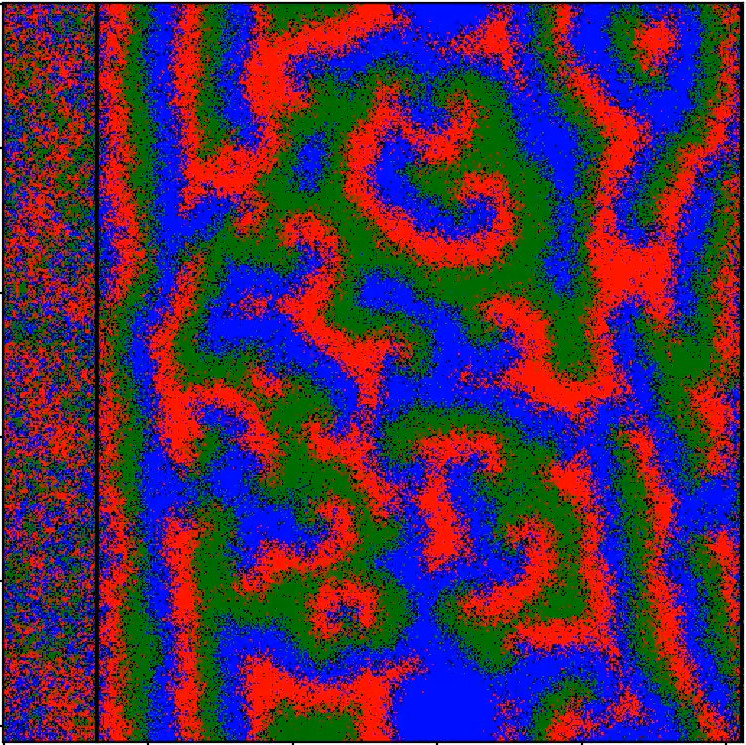
\includegraphics[width=0.45\linewidth]{images/RPS_2_5_ML_5.jpg}}
    \subfloat[ $ \delta_{\mathrm{CLV}} = 24.0 $ ]
    {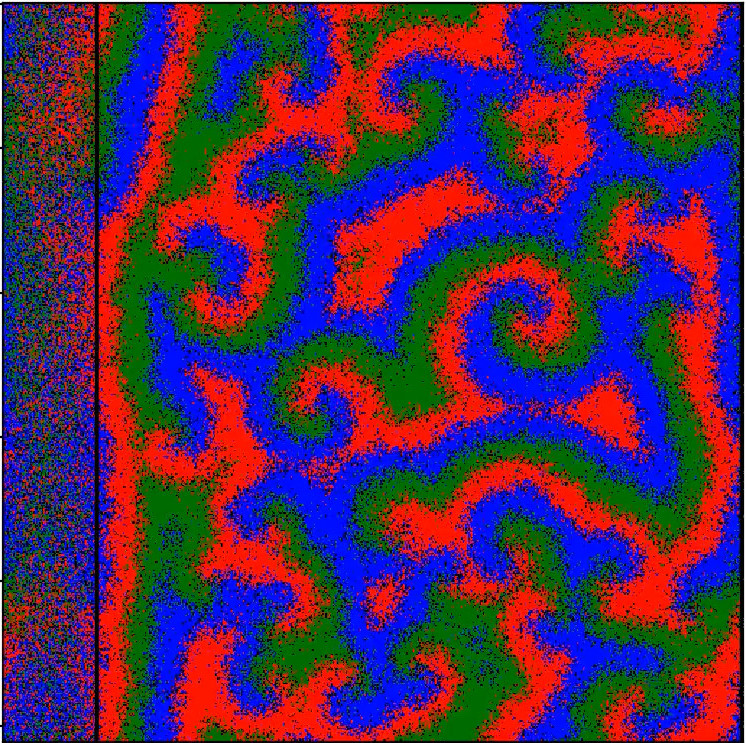
\includegraphics[width=0.45\linewidth]{images/RPS_24_ML_5.jpg}}\\
    \subfloat[ $ \delta_{\mathrm{CLV}} = 25.0 $ ]
    {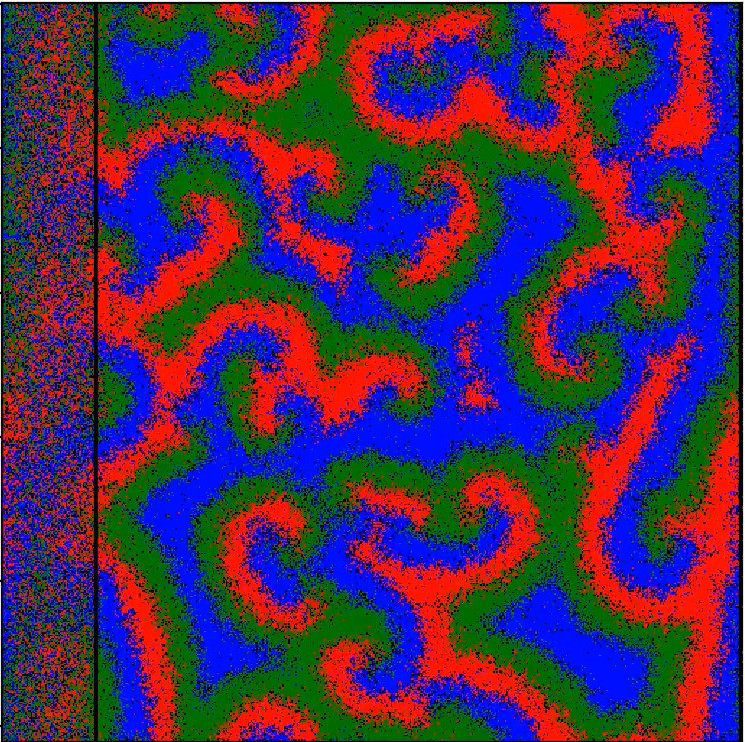
\includegraphics[width=0.45\linewidth]{images/RPS_25_ML_5.jpg}}
    \subfloat[ $ \delta_{\mathrm{CLV}} = 30.0 $ ]
    {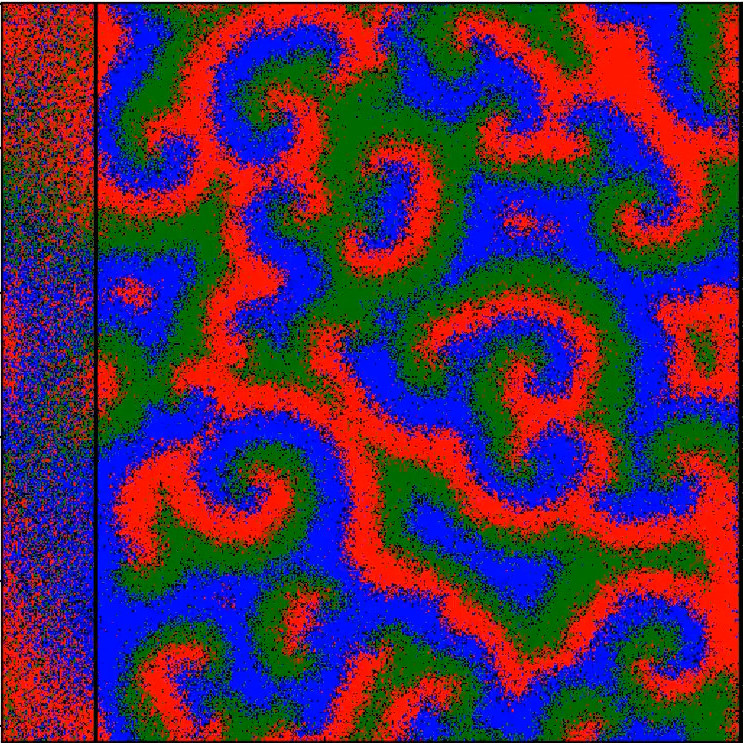
\includegraphics[width=0.45\linewidth]{images/RPS_30_ML_5.jpg}}
    \caption{Snapshots of combined CLVM and MLM systems on $ 512\times512 $ lattice with different values of $ \delta_{\mathrm{CLV}} $.
    The thick black line indicates the interface between the CLV and ML regions of the lattice.}
    \label{fig:plane_waves}
    \end{center} 
\end{figure}

\subsection{Plane-wave characterization}%
\label{sub:plane_wave}

We simulate the two-model system with $ \delta_{\mathrm{ML}} = 5.0 $ as at that value the pure ML model produces well defined
spiral waves that are small enough that several spirals fit on a $ 512\times512 $ lattice. When the CLVM and MLM are implemented on the same lattice, for values of $ \delta_{\mathrm{CLV}} $
below a certain value, the system displays a disruption of the spiral-wave patterns 
in the form of plane waves which travelaway from the interface. We observe that, with $ \delta_{\mathrm{ML}} = 5.0 $, the plane
waves begin to disappear at $ \delta_{\mathrm{CLV}} = 25.0 $.
The presence of these plane-waves is determined visually. 
We further quantify and characterize and quantify their behavior by calculating 
the vertical correlation length for each column of the system. 


\begin{figure}[!h]
    \begin{center}
    \subfloat[]
    {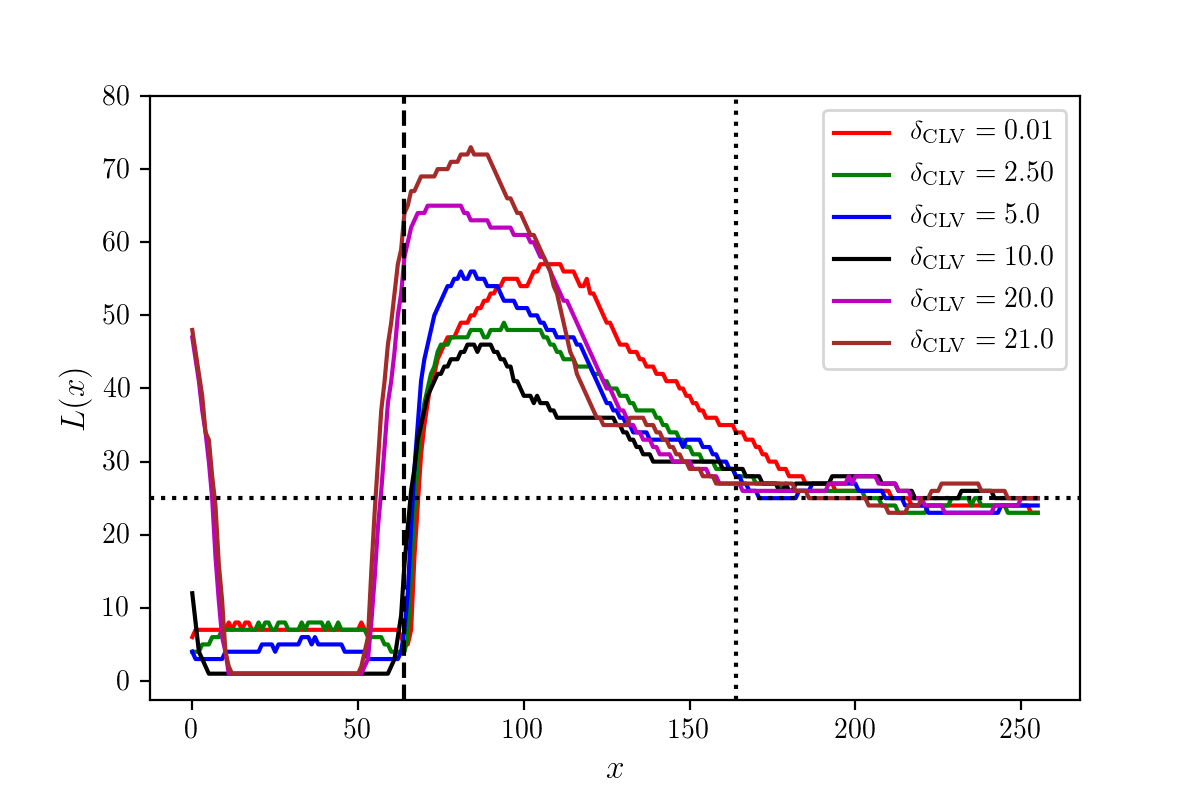
\includegraphics[width=0.75\linewidth]{images/corr_lens_3.png}}\\
    \subfloat[]
    {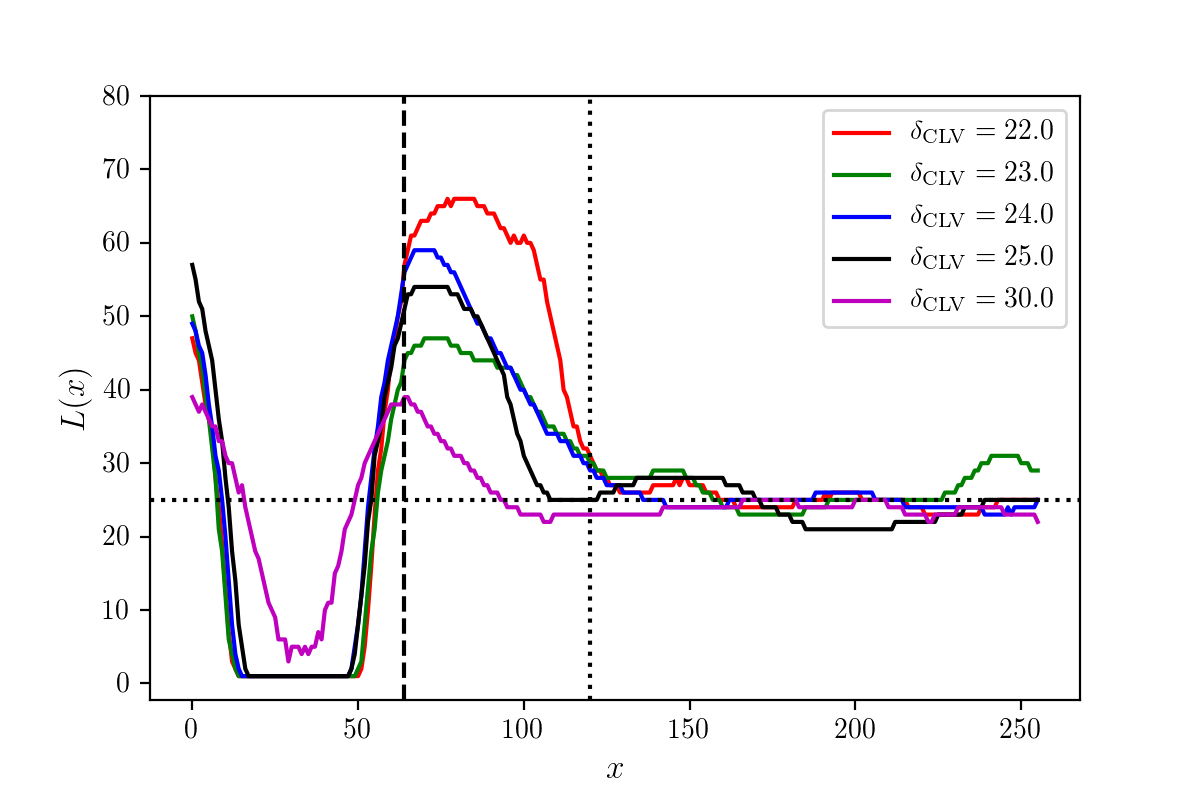
\includegraphics[width=0.75\linewidth]{images/corr_lens_4.png}}
    \caption{Vertical correlation lengths $ L(x) $ calculated for different values of $ \delta_{\mathrm{CLV}} $.
    The vertical dashed line indicates the interface between the CLV and ML regions of the lattice at $ x = 64 $ and the vertical 
    dotted lines are at $ x=164 $ and $ x = 120 $ in (a) and (b) respectively.  }
    \label{fig:corr_lens}
    \end{center} 
\end{figure}

We calculate the vertical two-point autocorrelation function for species $ j $ at time $ t $ 
\begin{equation}
    C_{jj}(r,x,t) = \frac{1}{M} \sum^{M}_{k=1} n_j(x, k, t)n_j(x, k+r, t) - \rho_j(x,t)^2
\end{equation}
where $ n_j(x,y,t) $ is the population of species $ j $ at the node $ \bm{x} = (x,y) $ and
$ \rho_j(x,t) = M^{-1} \sum_{k=1}^{M} n_j(x,k,t) $ is the population density of species $ j $
in column $ x $ of the lattice. Because of the cyclic symmetry inherent to RPS competition schemes,
we only calculate $ C_{jj} $ for $ j=1 $. We calculate $ \braket{C_{jj}(r,x)} $ by averaging $ C_{jj}(r,x,t) $ across 256 measurements 
taken every 4 MCS starting at $ t=3000  $ MCS (by which point the system has reached a (quasi-)steady state). 
$ \braket{C_{jj}(r,x)} $ is then finally averaged over 50 simulation runs. Using $ \braket{C_{jj}} $ we obtain
the vertical correlation length $ L(x) $ where $ L(x) $ is defined the least $ R $ for which 
$ \braket{C_{jj}(R,x)} $ is less than some threshold $ \epsilon $ (here taken to be $ 10^{-2} $). 

For values of $ \delta_{\mathrm{CLV}} $ for which plane waves are present (figure \ref{fig:corr_lens} (a), and the
red green and blue lines on figure \ref{fig:corr_lens} (b)) we observe an increase in $ L(x) $ near the interface
which returns to the MLM charcteristic length within 56-100 lattice sites of the interface. Notably, even for 
values of $ \delta_{\mathrm{CLV}} $ for which plane waves were not observed (the black and magenta plots in figure \ref{fig:corr_lens} (b))
we still see an increase in correlation lengths near the interface which disappears more quickly. Finally, we also 
observe an increase in $ L(x) $ in CLV region within approximately 15 lattice sites
of the interface for values of $ \delta_{\mathrm{CLV}} $ above 20.0.

\subsection{Population density}%
\label{sub:density}

\begin{figure}[h]
    \centering
    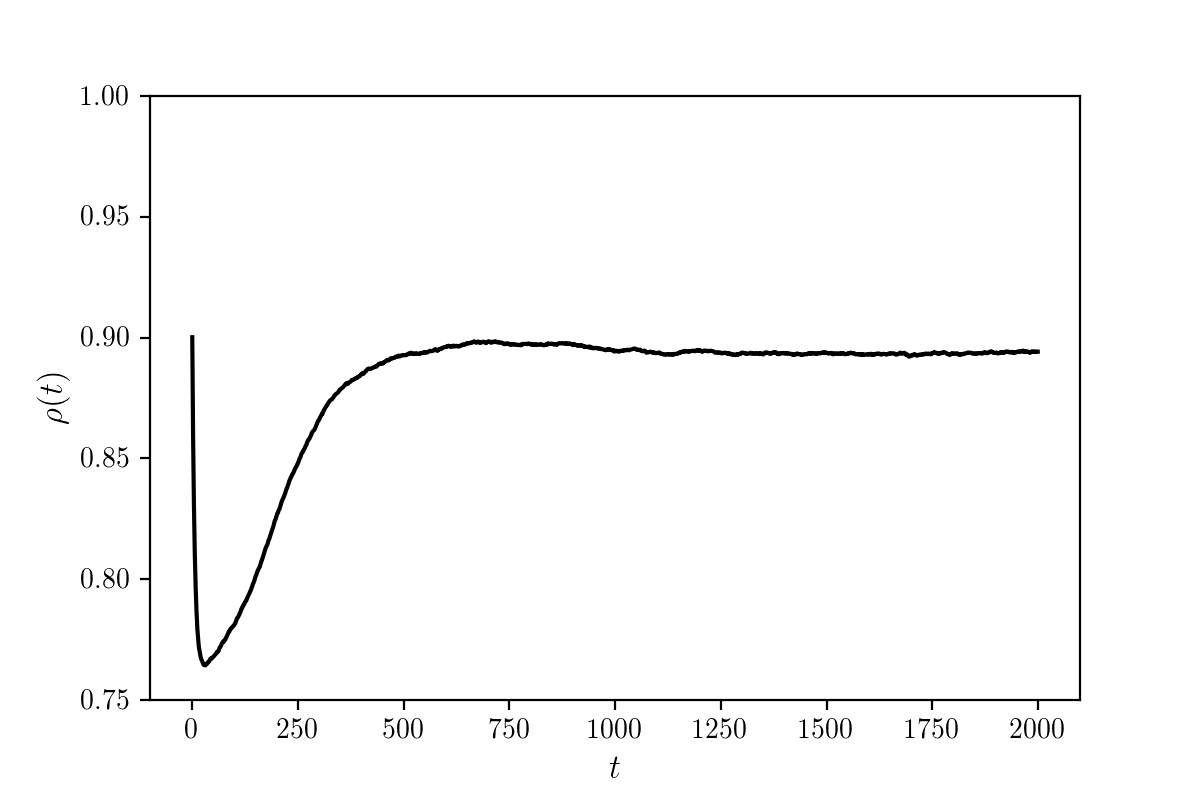
\includegraphics[width=0.8\linewidth]{images/net_density.png} 
    \caption{Global population density calculated for simulations of pure-ML systems. Averaged over 
    50 simulations.} \label{fig:net_den}
\end{figure}

It is established that spatially extended ML systems starting from randomized 
initial conditions exhibit an initial decline in global population density 
before spiral waves form, at which point predation is only possible at the border 
between species domain boundaries \cite{HeMobiliaTauber}. 
This causes the carrying capacity of the spatially-extended MLM to be greater than
that of a ``well mixed'' system. We replicate this result by computing the global population 
density $ \rho(t) = N^{-1} \sum_{j=1}^3\sum_{k=1}^{M}\sum_{l=1}^{M}n_j(l,k,t) $ for simulations of pure ML systems on a $ 256 \times 256 $ lattice (figure \ref{fig:net_den}).

\begin{figure}[h]
    \begin{center}
    \subfloat[]
    {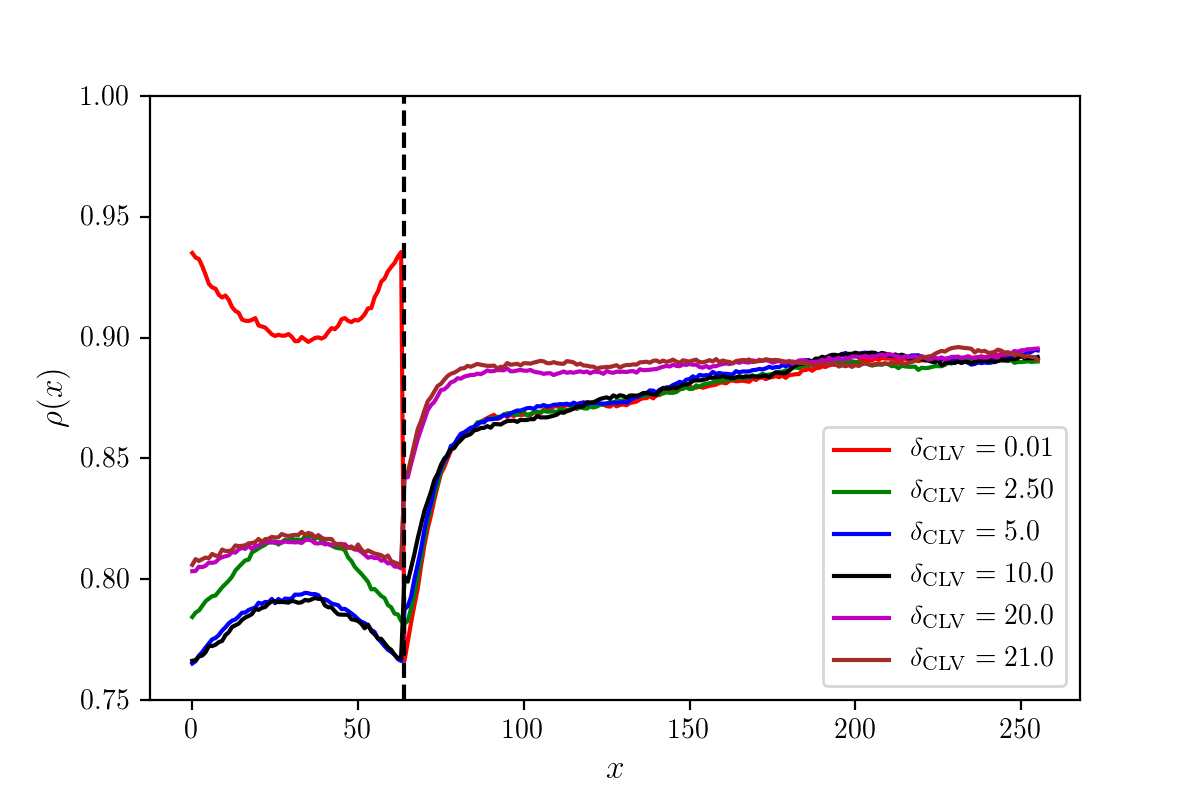
\includegraphics[width=0.75\linewidth]{images/den_1.png}}\\
    \subfloat[]
    {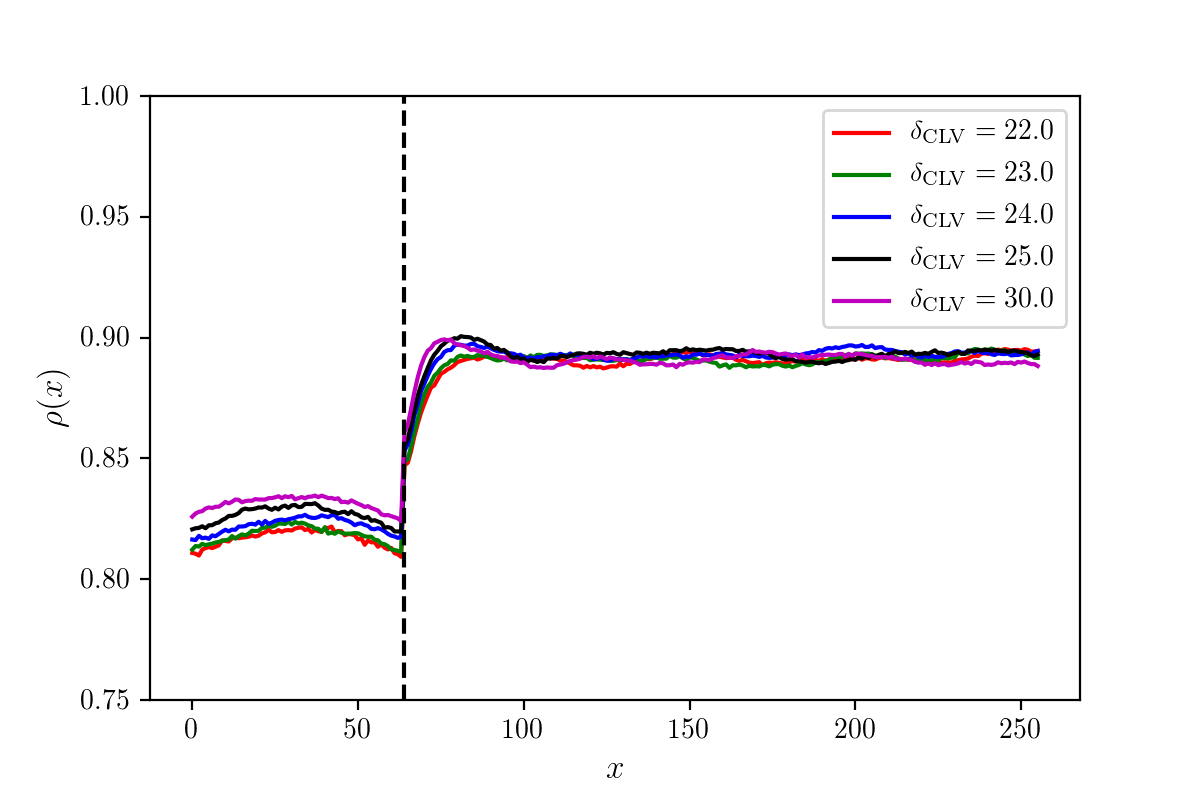
\includegraphics[width=0.75\linewidth]{images/den_2.png}}
    \caption{Vertical net population densities $ rho(x,t) $  calculated for different values of $ \delta_{\mathrm{CLV}} $.
    The vertical dashed line indicates the interface between the CLV and ML regions of the lattice at $ x = 64 $.}
    \label{fig:den}
    \end{center} 
\end{figure}

We compute the vertical net population density $ \rho(x,t) = M^{-1} \sum_{j=1}^3\sum_{k=1}^{M}n_j(x,k,t)$. $ \rho(x) $ is 
then calculated by averaging $ \rho(x,t) $ across 256 measurements taken every 4 MCS
starting at $ t=3000 $  MCS. $ \rho(x) $ is then averaged over 50 simulation runs. 
We observe a decrease in vertical population density near the interface (figure \ref{fig:den})
indicating that there is an increase in predation in $ ML $ region near the interface.
For low values of $ \delta_{\mathrm{CLV}} $ (the red plot in figure \ref{fig:den} (a))
the drop in local density is further enhanced by a net imbalance in migration between 
the two regions as indicated by the increase in density of the CLV region near
the interface. Note that the net density at the interface is less then both
the initialized denisty and the ML carrying capacity. This suggests that there 
is still some sort of ``well mixing'' effect allowing for increased predation at 
the interface despite the enhanced correlation length displayed in figure \ref{fig:corr_lens}.


\section{Discussion}%
\label{sec:conclusion}
In this paper, we demonstrate the appearance of plane-waves near the interface 
of mixed CLVM-MLM systems. We report an overall increase in vertical correlation
lengths near the interface across all values of $ \delta_{\mathrm{CLV}} $ tested.
As the value of $ \delta_{\mathrm{CLV}} $ is increased, the maximum distance from 
the interface at which the system still displays an increased correlation length
decreases. This suggests that, while there is still some disruption of the spiral-wave
formation occuring for higher values of $ \delta_{\mathrm{CLV}} $, it gives way 
quickly to the more stable spiral-waves. Furthermore, we report a decrease in local
population density near the interface indicating a local increase in predation. 
Overall, these results suggest localized periodic mixing as a means by which to
disrupt otherwise stable pattern formation in the MLM.

\bibliographystyle{abbrv}
\bibliography{biblio}





\end{document}

